\documentclass[a4paper,oneside]{article}
\usepackage[slovene]{babel}
\usepackage[utf8]{inputenc}
\usepackage{url}
\usepackage{graphicx}
\usepackage{epstopdf}
\usepackage[usenames]{color}
\usepackage[reqno]{amsmath}
\usepackage{amssymb}
\usepackage[bookmarks, colorlinks=true, %
linkcolor=black, anchorcolor=black, citecolor=black, filecolor=black,%
menucolor=black, runcolor=black, urlcolor=black%
]{hyperref}
\hypersetup{pdftitle={Iskanje optimalnega splošnega kompozitnega sortirnega algoritma}}
\hypersetup{pdfauthor={Jure Slak}}
\hypersetup{pdfsubject={Raziskovalna naloga}}
\usepackage[
    paper=a4paper,
    top=2.5cm,
    bottom=2.5cm,
%    textheight=24cm,
    textwidth=15cm,
    ]{geometry}


\usepackage{amsthm}
{
\newtheorem{izrek}{Izrek}[section]
\newtheorem{lema}[izrek]{Lema}
\newtheorem{trditev}[izrek]{Trditev}
\newtheorem{posledica}[izrek]{Posledica}
{
\theoremstyle{definition}
\newtheorem{definicija}{Definicija}[section]
}
}

\usepackage{listings}

\def\R{\mathbb R}
\def\N{\mathbb N}
\def\Z{\mathbb Z}
\def\C{\mathbb C}
\def\Q{\mathbb Q}

\usepackage{fancyhdr}
\pagestyle{fancy}

\title{Iskanje optimalnega splošnega kompozitnega sortirnega algoritma}
\author{Jure Slak}
\date{\today}

\begin{document}
\addto\captionsslovene {
\renewcommand\bibname{}
}
\renewcommand\refname{}

\lstset{language=c++, morekeywords={function, swap, to}}

%% naslovnica
\maketitle
\thispagestyle{empty}
\pagebreak

\tableofcontents
\pagebreak

\section{Uvod}

Sortiranje ali razvrščanje na splošno pomeni preurejanje dane množice objektov, na katerih
je definirana relacija linearne urejenosti, v vrstni red, določen s to relacijo.
Namen sortiranja je ponavadi olajšati kasnejše iskanje pripadnikov take urejene množice. Kot tako je
v vsesplošni uporabi in ima velik pomen. Objekti so sortirani v telefonskih imenikih,
davčnih registrih, stvarnih kazalih, knjižnicah, slovarjih, skladiščih in skoraj povsod tam,
kjer moramo shranjene predmete iskati in dosegati. Že majhne otroke učimo, da stvari spravljajo
``v red'' in tako z neke vrste sortiranjem prihajajo v stik daleč preden se naučijo kaj
aritmetike.

\subsection{Teoretični uvod}

%% refraziraj
%Sortiranje je torej pomembno in bistveno opravilo, še posebno v obdelavi podatkov. 
%Sortiranje je tudi idealen primer, na katerem prikažemo izredno raznolikost algoritmov,
%ki imajo vsi isti namen, od katerih so mnogi optimalni v nekem pomenu, in od katerih
%ima večina neko prednost pred ostalimi.

%% opis psevdokode

\subsubsection{Definicija algoritma}


\textbf{Algoritem} je končno zaporedje ukazov, ki, če jih ubogamo, opravijo neko nalogo.
Zanj velja:
\begin{itemize}
  \item \textbf{Ima podatke}. Množica podatkov je lahko tudi prazna.
  \item \textbf{Vrne rezultat}. Vrne vsaj eno izračunano vrednost ali kaj stori, kot na primer
    premakne papir na tiskalniku na novo stran.
  \item \textbf{Je natančno določen}. Vsak ukaz mora nedvoumno povedati kaj storiti.
  \item \textbf{Se vedno konča}. Končati se mora pri vseh možnih naborih vhodnih podatkov.
  \item \textbf{Mogoče ga je opraviti}. V načelu ga je mogoče izpeljati ``peš'', s papirjem in
    svinčnikom.
\end{itemize}
% citat [KOZ86], str 11


\begin{definicija}
  Algoritem je \textbf{kompoziten} oziroma \textbf{sestavljen}, če je sestavljen iz večih
  drugih algoritmov.
\end{definicija}


\subsubsection{Definicija sortiranja}
Naj bo dan končen vektor elementov $\vec{a} = \left(a_1, a_2, \ldots a_n \right)$ in relacija $\leq$.
Naj bo $f(a)$ \emph{ključ} elementa. Definirana mora biti relacija linearne urejenosti med 
ključi elementov.V splošnem je dana relacija $\leq$ med elementi $\vec{a}$-ja, ki je definirana kot 
\[a_i \leq a_j \overset{def}{\Longleftrightarrow} f(a_i) \leq f(a_j). \]

$f$ je ponavadi trivialen, ker je $f(a)$ ponavadi kar del $\vec{a}$-ja in nam ga ni treba
računati, lahko pa to ni res. 

Definirajmo še tip \emph{item}, ki naj ponazarja elemente $\vec{a}$-ja. Naj bo \emph{key}
ključ elementa tipa \emph{cmp\_t}, na katerem je definirana relacija linearne urejenosti.

\begin{lstlisting}
struct item {
    cmp_t key;
    /* ostale komponente */
};
\end{lstlisting}

Ostale komponente predstavljajo s stališča urejanja nepomembne podatke o elementih v zbirki
S stališča sortirnih algoritmov je ključ \emph{edini} pomemben podatek in torej ni treba
podrobno definirati drugih komponent.

\begin{definicija}
  \textbf{Sortirni algoritem} je algoritem, ki prejme neko podatkovno strukturo s podatki
  in jih uredi po nekem vrstnem redu.
\end{definicija}

\begin{definicija}
  Sortirnemu algoritmu pravimo, da je \textbf{stabilna}, če ostane po končanem sortiranju
  relativni vrsti red elementov z istim ključem nespremenjen.
  Stabilnost sortiranja je pogosto zaželena, če so elementi že urejeni po neki
  sekundarni $\leq$ relaciji, torej glede lastnosti, ki jih (primarni) ključ ne izraža.
\end{definicija}

\begin{definicija}
  O neki sortirni metodi pravimo, da se dogaja \textbf{na mestu}, če se med izvajanjem podatki, ki
  jih sortiramo, ne kopirajo v dodaten pomnilnik.
\end{definicija}

\begin{definicija}
  Sortirni algoritem je \textbf{primerjalen}, če ureja elemente tako, da jih primerja med seboj.
\end{definicija}


Vsi nadaljnji algoritmi bodo definirani kot procedure s tremi parametri, $a$, $prvi$,
$zadnji$, ki predstavljajo:
\begin{itemize}
  \item $a$: polje, ki ga sortiramo. V splošnem zahtevamo, da je to katerakoli podatkovna
    struktura, ki $a$ podpira neko vrsto naključnega dostopa. Le-tega uporabljamo, kadar 
    uporabljamo operator $[\cdot]$. Zaradi časovne analize algoritmov zahtevamo, da operator 
    $[\cdot]$ deluje v konstantnem času. Indeksiranje elementov polja se začne z 0.
    V nadaljnjem opisovanju bom uporabljal besedo
    polje za katerokoli podatkovno strukturo, ki ustreza zgornjim zahtevam.
  \item $prvi$: indeks prvega elementa, ki ga želimo sortirati.
  \item $zadnji$: indeks elementa, ki je za zadnjim elementom, ki ga sortiramo. Lahko ni
    veljaven indeks v $a$.
\end{itemize}
Vse procedure bodo spremenile polje $a$, nobena ne bo ničesar vrnila.

Pri definiciji časovne in prostorske zahtevnosti algoritma bo za prostorsko zahtevnost 
navedena zgolj dodatna poraba pomnilnika, saj vsi algoritmi porabijo $O(n)$ pomnilnika za
shranjevanje celotnega polja, kjer $n$ predstavlja število elementov v polju, ali razliko
$zadnji - prvi$. 

\subsubsection{Urejanje z navadnim vstavljanjem}
Urejanje z navadnim vstavljanjem\footnote{vir: IJS-jev slovar računalniških izrazov
\url{http://www.ijs.si/cgi-bin/rac-slovar}} (\emph{angl.} insertion sort) je metoda,
podobna tisti, ki jo na široko uporabljajo igralci kart. Je primerjalni sortirni algoritem.

Zaporedje $a_1, a_2, \ldots, a_n$ razdelimo na že urejeni del $a_1, a_2, \ldots, a_{i-1}$
in še neurejeni del $a_i, \ldots a_n$. Nato $a_i$ vstavimo na pravo mesto v že sortirani
del. Ponovimo z $i + 1$. Začnemo z $i = 2$, ko je prvi del trivialno sortiran, saj ima le
en element.

Elemente miselno razdelimo na končno zaporedje $a_0, a_1, \ldots,
a_{i-1}$ in na začetno zaporedje $a_i,\ldots, a_n$. Na vsakem koraku začenši z $i = 1$ in
prirastkom ena, vstavimo $i$-ti element začetnega zaporedja na ustrezno mesto v končnem
zaporedju.

\begin{figure}[h]
    \begin{center}
        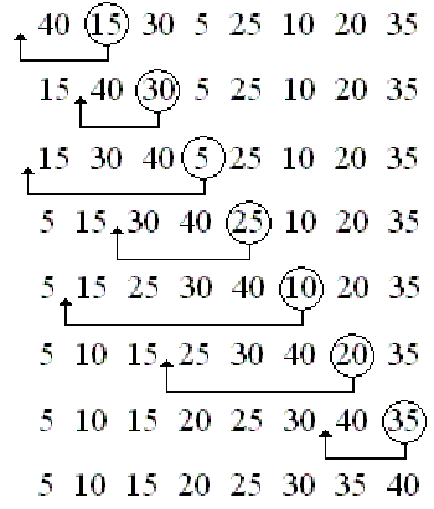
\includegraphics[height=45mm]{slike/insertionsort.png}
    \end{center}
    \caption{Grafična predstavitev urejanja z navadnim vstavljanjem.}
    \label{fig:insertion-sort-predst}
\end{figure}

Postopek sortiranja z navadnim vstavljanjem je prikazan na primeru osmih naključno
izbranih števil (glej sliko \ref{fig:insertion-sort-predst}). Algoritem navadnega
vstavljanja lahko zapišemo v psevdokodi nekako tako (sortira se vse na intervalu
$\left[prvi, zadnji\right)$):

\lstinputlisting{insertionsort.code}

Med postopkom iskanja pravega mesta je dobro sproti premikati elemente med izvajanji
primerjanj. Z drugimi besedami, pustiti $x$, da se ``pogrezne'' tako, da $x$
primerjamo z naslednjim elementom $a_j$ in ga bodisi vstavimo, če je ključ $a_j$ manjši
ali enak $x$ ali pa $a_j$ premaknemo na desno ter nadaljujemo proti levi, če še nismo pri
levem robu polja. Postopek ``pogrezanja'' lahko ustavita ta dva ločena
pogoja, kot je prikazano v zgornji \emph{while} zanki.  Ko vstavimo še zadnji element v že 
urejeno zaporedje, smo z urejanjem zaključili.\\

\textbf{Časovna in prostorska zahtevnost}. \\
Časovna zahtevnost je v 
\begin{itemize}
  \item najboljšem primeru $O(n)$
  \item povprečnem primeru $O(n^2)$
  \item najslabšem primeru $O(n^2)$
\end{itemize}

Prostorska zahtevnost je v vsakem primeru $O(1)$, saj se vse premene dogajajo na
mestu.\newline

Spodnja časovna meja ustreza primeru, ko so elementi na začetku že urejeni, zgornja pa primeru,
ko so elementi na začetku nasprotno urejeni. Podani algoritem opisuje tudi stabilen postopek sortiranja, kajti medsebojni
vrstni red elementov z enakimi ključi ostane nespremenjen.

Urejanje z navadnim vstavljanjem je zelo učinkovito na majhnih poljih. Učinkovito je tudi na že
skoraj sortiranih poljih, saj se s tem približujemo obnašanju v najboljšem primeru.
Zaradi kvadratne časovne zahtevnosti je urejanje z navadnim vstavljanjem zelo neučinkovito na
dolgih poljih, če ta niso že skoraj urejena.

\subsubsection{Hitro urejanje}
Hitro urejanje ali urejanje s porazdelitvami\footnote{vir: IJS-jev slovar računalniških izrazov
\url{http://www.ijs.si/cgi-bin/rac-slovar}} (\emph{angl.} quicksort) je eden izmed
najučinkovitejših sortirnih algoritmov, ki jih poznamo, razvil pa ga je C. A. R. Hoare.
Je primerjalni sortirni algoritem, ki uporablja metodo deli in vladaj.

Sortiranje s porazdelitvami temelji na dejstvu, da moramo premene opravljati na večje
razdalje, da bi bile najučinkovitejše. Recimo, da imamo $n$ nasprotno urejenih elementov.
V tem primeru jih lahko sortiramo z le $n/2$ premenami tako, da najprej premenjamo prvega
in zadnjega in se postopoma pomikamo proti sredini. Seveda je to možno le, če vemo, da so 
elementi natanko nasprotno urejeni.

Prejšnji primer nas napelje na naslednji algoritem: 
zberemo poljuben element (recimo mu pivot in ga označimo z $x$), nato začnemo 
polje pregledovati z leve, dokler ne najdemo elementa $a_i > x$ in nato z desne dokler ne 
najdemo elementa $a_i < x$. Elementa sedaj medsebojno zamenjamo in nadaljujemo s 
pregledovanjem in premenami, dokler se ne srečamo nekje na sredi polja.
Polje je sedaj razdeljeno na levi del s ključi manjšimi od $x$ in na desni del
s ključi večjimi od $x$. Metodo ponovimo na obeh delih dokler ne pridemo do že urejenih
podpolj. 

Iz prejšnjega algoritma ugotovimo, da je izbira pivota zelo
pomembna. Pogosto je, da za pivot vzamemo kar zadnji element, vendar to sproži ravno
najslabšo možnost izvajanja programa, če so elementi že urejeni. Zato sem v svoji
implementaciji za pivot vzel mediano prvega, srednjega in zadnjega elementa oziroma t.i.
mediano treh. Pogosta izbira je tudi naključni pivot. 

Postopek sortiranja s porazdelitvami je prikazan na primeru devetih naključno
izbranih števil (glej sliko \ref{fig:quick-sort-predst}). Izbrani pivoti so obarvani sivo.
Vsaka vrstica predstavlja svojo globino rekurzije.

%% definicija rekurzije ?kam, kje jo dobim?

\begin{figure}[h]
    \begin{center}
        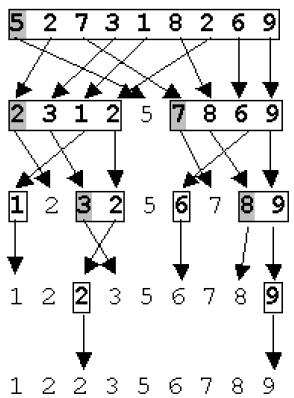
\includegraphics[height=45mm]{slike/quicksort.jpg}
    \end{center}
    \caption{Grafična predstavitev urejanja s porazdelitvami.}
    \label{fig:quick-sort-predst}
\end{figure}

V psevdokodi bi zapisali algoritem urejanja s porazdelitvami
nekako tako (sortira se vse na intervalu
$\left[prvi, zadnji\right)$):
Predpostavimo, da obstaja funkcija \emph{swap}, ki zamenja vrednosti dveh spremenljivk.

\lstinputlisting{quicksort.code}

\textbf{Časovna in prostorska zahtevnost}. \\
Časovna zahtevnost je v 
\begin{itemize}
  \item najboljšem primeru $O(n\log_2 n)$
  \item povprečnem primeru $O(n\log_2 n)$
  \item najslabšem primeru $O(n^2)$
\end{itemize}

Prostorska zahtevnost je v najboljšem in povprečnem primeru $O(\log_2 n)$, 
saj algoritem opravlja premene na mestu, vsak rekurziven klic pa zahteva $O(1)$ prostora.
V najslabšem primeru je rekurzivnih klicev $n$, zato zahteva algoritem $O(n)$ prostora.

Urejanje s porazdelitvami je eden najhitrejših sortirnih algoritmov, kar jih
poznamo. Svojo hitrost dolguje arhitekturi današnjih procesorjev, ki imajo
malo registrov in precej notranjega pomnilnika, saj lahko pivot ponavadi shranimo v
register, kar prihrani veliko poizvedb do pomnilnika. Dober je na enakomerno
porazdeljenih podatkih, a kljub pazljivemu izbiranju pivotov obstaja možnost neželenega
najslabšega primera, čeprav je zelo neverjetna. 

\subsubsection{Urejanje s kopico}
Urejanje s kopico\footnote{vir: IJS-jev slovar računalniških izrazov
\url{http://www.ijs.si/cgi-bin/rac-slovar}} (\emph{angl.} heapsort) je sortirni algoritem,
ki si pri sortiranju pomaga s kopico.
\newline

Kopica je urejena drevesna podatkovna struktura.
Maksimalno kopico definiramo kot zaporedje ključev $h_i, h_{i+1}, \ldots, h_n$, pri čemer
velja
\begin{align*}
  h_i &\geq h_{2i} \\
  h_i &\geq h_{2i+1}
\end{align*}
pri vseh $i = 1 \ldots n/2$. %% r sem zamenjal z n?? pa tudi tu je treba vzeti celi del n/2
Kopico lahko predstavimo v polju, kjer je koren kopice na mestu 1, in velja, da sta otroka
starša na mestu $i$, na mestih $2i$ in $2i + 1$.

Urejanje s kopico podatke najprej preuredi v maksimalno kopico. Nato odstrani koren kopice
-- največji element in ga zamenja z zadnjim elementom kopice. Potem ponovno ustvari
maksimalno kopico na preostanku elementov in zopet odstrani korenski element ter ga
zamenja s tistim na predzadnjem mestu. To se ponavlja dokler ni kopica dolga le en
element. 

Urejanje s kopico je prikazano na sliki \ref{fig:heap-sort-predst}.
Vsaka črta predstavlja svoj element, večji ko je element, temnejša je črta.
Do rdečega zaznamka na dnu slike poteka urejanje podatkov v kopico, nato pa odstranjevanje
največjega elementa in ponovna vzpostavitev kopice vse ko konca.
\begin{figure}[h]
    \begin{center}
        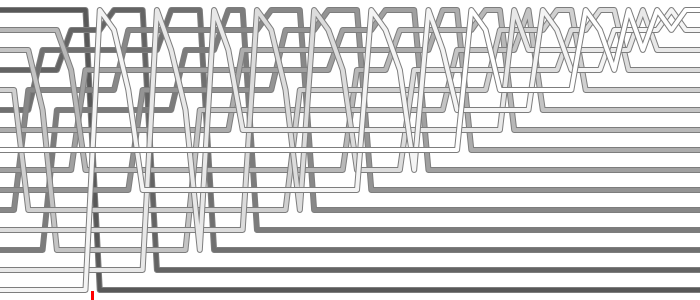
\includegraphics[height=45mm]{slike/Heap.png}
    \end{center}
    \caption{Grafična predstavitev urejanja s kopico.}
    \label{fig:heap-sort-predst}
\end{figure}


V psevdokodi bi algoritem urejanja s kopico izgledal nekako tako (sortira se vse na intervalu
$\left[prvi, zadnji\right)$):
Predpostavimo, da obstaja funkcija \emph{swap}, ki zamenja vrednosti dveh spremenljivk.

\lstinputlisting{heapsort.code}

%% zakaj ni čšž-jev

\textbf{Časovna in prostorska zahtevnost}. \\
Časovna zahtevnost je v najboljšem, povprečnem in najslabšem primeru $O(n\log_2 n)$.

Prostorska zahtevnost je v vsakem primeru $O(1)$, saj je kopica predstavljena kar v
seznamu, ki ga urejamo, in ker se vse premene dogajajo na mestu.

Čas izvajanja urejanja s kopico je neodvisen od morebitne urejenosti podatkov v polju,
kot lahko razberemo iz časovne zahtevnosti. Zaradi dokaj zapletenega postopka sortiranja,
na manjših poljih ni tako uspešen, je pa čedalje bolj uspešen, ko se dolžina polja
povečuje.

\subsubsection{Urejanje z zlivanjem}
Urejanje z zlivanjem (\emph{angl.} merge sort) je primerjalni sortirni algoritem, ki
uporablja metodo deli in vladaj. Odkril ga je John von Neumann leta 1945.
Urejanje z zlivanjem uporablja idejo, da je v sortirano polje hitreje združiti dve že
sortirani polji, kot pa dve še ne sortirani. 
Algoritem urejanja z zlivanjem ureja tako:
\begin{enumerate}
  \item Če je polje dolgo 0 ali 1 je že sortirano, če ne:
  \item Razdeli polje v dve približno enako dolgi podpolji
  \item Sortiraj podpolji 
  \item Združi podpolji nazaj v celotno sortirano polje.
\end{enumerate}

Algoritem je grafično prikazan na sliki \ref{fig:merge-sort-predst} na primeru sedmih
naključno izbranih števil.
Vsaka vrstica števil predstavlja svojo globino rekurzije, vse dokler niso polja dolga le
po en element. Nato se začne izvajati četrta točka algoritma, ponazorjena z vrsticami
nižje od črtkane črte, ki združi podpolja v sortirano polje.

\begin{figure}[h]
    \begin{center}
        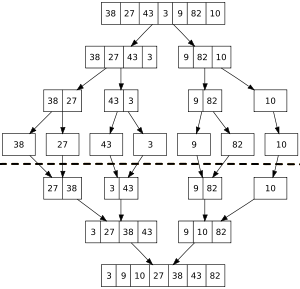
\includegraphics[height=55mm]{slike/merge_sort.png}
    \end{center}
    \caption{Grafična predstavitev urejanja z zlivanjem.}
    \label{fig:merge-sort-predst}
\end{figure}

V psevdokodi bi ta algoritem zapisali nekako tako (sortira se vse na intervalu
$\left[prvi, zadnji\right)$):
\lstinputlisting{mergesort.code}

\textbf{Časovna in prostorska zahtevnost}. \\
Časovna zahtevnost je v najboljšem, povprečnem in najslabšem primeru $O(n\log_2 n)$.

Prostorska zahtevnost je v vsakem primeru $O(n)$. % ker O(n + log n)

Časovna zahtevnost urejanja z zlivanjem ni odvisna od morebitne že delne urejenosti ali
neurejenosti podatkov v polju. V praksi je urejanje z zlivanjem najbolj učinkovito na
sekvenčnih medijih kot na primer tračnih enotah ali podatkovnih strukturah, ki nimajo hitrega
neposrednega dostopa do nekega elementa z njegovim indeksom, kot na primer povezani seznami.

\subsubsection{Bisekcija}
Bisekcija je postopek za iskanje ničel zveznih funkcij. Podrobneje je opisana v
\cite{bib:bohte91}.
Če imamo zvezno funkcijo, ki je v točki $a$ pozitivna, v točki $b$ pa
negativna nam izrek o bisekciji zagotavlja, da ima funkcija na tem 
intervalu vsaj eno ničlo. To ničlo poiščemo rekurzivno:
pogledamo, kakšnega predznaka je funkcija v točki $\frac{a+b}{2}$. Če smo našli
ničlo, smo končali. Če je funkcija pozitivna, nadaljujemo na intervalu
$\left[\frac{a+b}{2}, b\right]$, če ne, pa na intervalu $\left[a, \frac{a+b}{2}\right]$, saj ta
interval izpolnjuje pogoje izreka. Končamo, ko je $\left(a-b\right)$ manjša od želene natančnosti.

\subsubsection{Graf}
\textbf{Graf} sestavljata dve množici, $V$ in $P$. $V$ je končna neprazna množica vozlišč
ali točk, $P$ pa množica parov vozlišč. Elementom množice $P$ pravimo povezave, celotni
graf pa označimo z $G = (V, P)$.

Graf je lahko \textbf{neusmerjen} ali \textbf{usmerjen}. V prvem primeru par vozlišč, ki sestavljata
povezavo, ni urejen, v drugem pa je prvo od vozlišč začetek, drugo pa konec povezave.
Neusmerjenemu grafu, v katerem je poljubno vozlišče povezano z vsemi ostalimi, pravimo
polni graf. 

\textbf{Pot} je zaporedje povezav $\left(v_{i_1}, v_{i_2}\right), \left(v_{i_2},
v_{i_3}\right), \ldots, \left(v_{i_{r-1}}, v_{i_r}\right)$. Naslednja povezava v poti se
začenja tam, kjer se je prejšnja končala. Pot je \textbf{enostavna}, če gre skozi vsako
vmesno vozlišče le enkrat. Zaključena enostavna pot je \textbf{cikel}.
Grafu v katerem ni ciklov pravimo \textbf{acikličen}. Graf je \textbf{povezan}, če obstaja
pot iz poljubnega vozlišča v poljubno drugo vozlišče.

Graf lahko predstavimo z matriko sosednosti in s seznamom sosedov.
Naj $n$ označi število vozlišč v grafu. Vozlišča najpreprosteje označimo kar z indeksom $i,
i = 1, 2, \ldots, n$. Z matriko sosednosti $A := (a_{ij})$ bomo graf predstavili z 

\[ a_{ij} := 
\left\{
\begin{array}{ll}
  1,& (i, j) \in P, \\
  0,& (i, j) \notin P, i, j = 1, 2, \ldots, n. 
\end{array}
\right. %% wtf?
\]
 
\begin{figure}[h]
    \begin{center}
        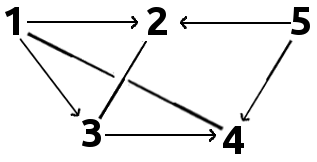
\includegraphics[height=25mm]{slike/graf1.png}
    \end{center}
    \caption{Primer grafa.}
    \label{fig:graf1}
\end{figure}

Predstavitev grafa na sliki \ref{fig:graf1} z matriko sosednosti bi bila sledeča:

\[
A = \left(
\begin{array}{ccccc}
  0 & 1 & 1 & 1 & 0 \\
  0 & 0 & 1 & 0 & 0 \\
  0 & 1 & 0 & 1 & 0 \\
  1 & 0 & 0 & 0 & 0 \\
  0 & 1 & 0 & 1 & 0 \\
\end{array}
\right)
\]

Predstavitev z matriko nam ponuja še možnost shranjevanja dodatne informacije. Vzemimo, da
za vsako povezavo v grafu poznamo še en podatek, na primer dolžino ali vrednost povezave.
Dolžino lahko zapišemo kar v matriko, če se le dogovorimo, kakšno dolžino imajo povezave,
ki jih ni. Najpogosteje bomo uporabili dogovor, da je dolžina neskončna.
\pagebreak
\begin{figure}[h]
    \begin{center}
        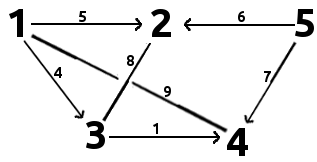
\includegraphics[height=25mm]{slike/graf2.png}
    \end{center}
    \caption{Primer grafa s podanimi dolžinami povezav.}
    \label{fig:graf2}
\end{figure}


Graf na sliki \ref{fig:graf2} bi z matriko predstavili tako:

\[
A = \left(
\begin{array}{ccccc}
  \infty & 5      & \infty & 9      & \infty \\
  \infty & \infty & 8      & \infty & \infty \\
  \infty & 8      & \infty & 1      & \infty \\
  9      & \infty & \infty & \infty & \infty \\
  \infty & 6      & \infty & 7      & \infty \\
\end{array}
\right)
\]

Prostorska zahtevnost predstavitve grafa na tak način je $O(n^2)$. Zato bo primerna
predvsem tedaj, ko je graf blizu polnemu in imamo res $O(n^2)$ podatkov.

Turnirji so zanimivi.

\subsection{Nameni in cilji}
\subsection{Hipoteze}
\begin{enumerate}
  \item Kompoziten algoritem se odnese boljše na različnih tipih podatkov kot vsak
    posamezen algoritem.
\end{enumerate}
\section{Metode dela}
Za preverjanje hipotez(e) sem si izbral eksperiment, saj se mi zdi da je to edina metoda
dela, s katero je hipotezo sploh mogoče preverjati in pa delo z viri, ki sem jih
potreboval pri pripravi eksperimenta.
Za izvedbo eksperimenta sem implementiral vse v teoretičnem delu opisane sortirne
algoritme. Za implementacijo sem si izbral programski jezik C++, predvsem zaradi njegove
hitrosti in še česa. %% hja česa?

Vsak izmed sortirnih algoritmov je implementiran kot funkcija z dvema parametorma.
Vsaka funkcija sprejme dva Random Access iteratorja, %%
ki kažeta na prvi element, ki ga sortiramo in na prvi element za tistim, ki ga sortiramo
zadnjega. Slednji je lahko neveljaven v polju (kaže preko njenega konca).
Tako obliko funkcij sem si izbral predvsem zato, ker je v sladu z zapisom, ki ga uporablja
C++-ov header algortihm. Drugi razlog je, da s tem zapisom dosežemo minimalno število
parametrov pri trenutni funkcionalnosti. Če bi želeli le en parameter, bi bilo to
izvedljivo, vendar bi se morali odpovedati zmožnosti, da lahko sedaj sortiramo le željeni
del polja. V primeru zgolj enega parametra to ne bi bilo možno, vedno bi se
sortiralo celotno polje.

% more to be written
%
% problem s stringi


\section{Rezultati}
\section{Ugotovitve in razprava}
\section{Sklep}
Potrdili smo hipotezo. Lahko bi izboljšali z bolj optimizirano implementacijo.
\section{Zaključek}
Zadeva je uporabna.
\section{Viri in Literatura}
\subsection{Literatura}
\vspace{-1cm}
\begin{thebibliography}{99}
  \bibitem[BOH91]{bib:boh91} {Z. Bohte, \emph{Numerične metode, 4.\ ponatis}. DMFA Slovenije, Ljubljana 1991.}
    %% tega nimam in nevem kje nej dobim
  \bibitem[KOZ86]{bib:koz86} {J. Kozak, \emph{Podatkovne strukture in algoritmi}. DMFA SRS, Ljubljana 1986. }
\end{thebibliography}
\subsection{Priloge}


\end{document}
% vim: spell spelllang=sl
